\documentclass[journal,transmag]{IEEEtran}

\usepackage{cite}
\usepackage[pdftex]{graphicx}
\graphicspath{{./Figures/}}
\DeclareGraphicsExtensions{.pdf,.jpeg,.png,.jpg}
\usepackage{caption}
\usepackage{amsmath}
\interdisplaylinepenalty=2500
\usepackage{algorithmic}
\usepackage{array}
\usepackage[caption=false,font=normalsize,labelfont=sf,textfont=sf]{subfig}
\usepackage{dblfloatfix}
\usepackage{url}
\usepackage{lipsum}
\usepackage{xcolor}
\usepackage{listings}


\lstset{
	escapeinside={/*@}{@*/},
	language=Java,	
	basicstyle=\fontsize{8.5}{12}\selectfont,
	numbers=left,
	numbersep=2pt,    
	xleftmargin=2pt,
	frame=tb,
	columns=fullflexible,
	showstringspaces=false,
	tabsize=4,
	keepspaces=true,
	showtabs=false,
	showspaces=false,
	morekeywords={inline,public,class,private,protected,struct},
	captionpos=b,
	lineskip=-0.4em,
	aboveskip=10pt,
	extendedchars=true,
	breaklines=true,
	prebreak = \raisebox{0ex}[0ex][0ex]{\ensuremath{\hookleftarrow}},
	keywordstyle=\color[rgb]{0,0,1},
	commentstyle=\color[rgb]{0.133,0.545,0.133},
	stringstyle=\color[rgb]{0.627,0.126,0.941},
}

% correct bad hyphenation here


\begin{document}

\title{An Investigation into the Speed-up of a Ray Tracer Application via the use of OpenMP and MPI}

\author{\IEEEauthorblockN{Sam Dixon \\ 40056761@live.napier.ac.uk}
\IEEEauthorblockA{SET10108 - Concurrent and Parallel Systems \\ School of Computing,
Edinburgh Napier University, Edinburgh}% <-this % stops an unwanted space

\thanks{Project available at: github.com/neaop/SET10108Coursework\_2}}


\markboth{SET10108 - Coursework 2}{}
% The only time the second header will appear is for the odd numbered pages after the title page when using the twoside option.

\IEEEtitleabstractindextext{
\begin{abstract}
	The abstract goes here.
\end{abstract}

\begin{IEEEkeywords}
	C++11, Ray Tracer, Parallel, OpenMP, MPI, Speed-up.
\end{IEEEkeywords}}

\maketitle

\IEEEdisplaynontitleabstractindextext

\IEEEpeerreviewmaketitle

\section{Introduction}
 
	\IEEEPARstart{T}{he} aim of this report is to document and analyse the results of an attempt to speed-up a C++11 Ray tracer application - via the use of concurrency and parallelisation techniques. The methods being tested in this project are \texttt{OpenMP} and \texttt{MPI}.
	
	\subsection{Ray Tracing}
		Ray Tracing a rendering technique that allows an image to be generated by tracing the path of a ray of light and simulating the effects that a virtual environment have upon it.
			
			\begin{figure*}[]
				\centering
				\subfloat[Four Samples per Pixel]{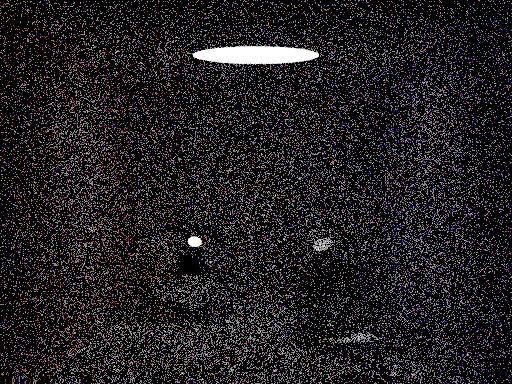
\includegraphics[width=2.5in]{raytracerPPM4}%
					\label{fig_first_case}}
				\hfil
				\subfloat[Four-hundred Samples per Pixel]{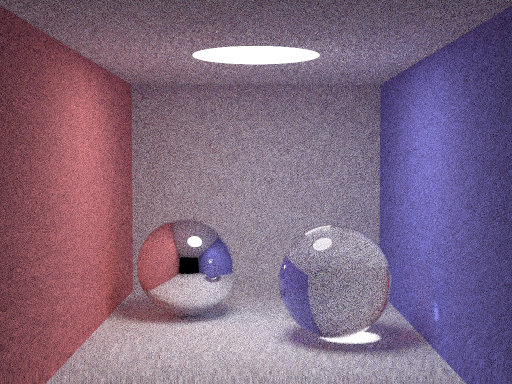
\includegraphics[width=2.5in]{raytracerPPM400}%
					\label{fig_second_case}}
				\caption{Two images produced by the Ray Tracer.}
				\label{fig_sim}
			\end{figure*}
		
	\subsection{OpenMP}
		\texttt{OpenMP} (Open Multi-Processing) is an open source API that allows for the implementation of shared memory multiprocessing with minimal developmental effort. \texttt{OpenMP} makes use of the C++ \texttt{\#pragma} directive and the pre-processor to allow developers to flag sectors of code to be parallelised. A number of different scheduling options can be implemented to alter the way in which \texttt{OpenMP} parallelises an application.

	\subsection{MPI}
		\texttt{MPI} (Message Passing Interface) is a standardised method of distributed parallelism that operates by having multiple processors communicate by sending and receiving signals from one another via communication channels. 
		
\section{Methodology}
	
	\subsection{Profiling}
		Prior to implementing any methods that will save time, the sequential code must first be analysed. By using the Visual Studio Performance Profiler, it is possible to evaluate the sequential code and locate the functions or methods that use up the most CPU time. Once the potentially problematic areas have been identified, a suitable parallelisation method can be implemented to reduce the impact of those areas on the execution time. It should be noted that all code presented in the report was run without any form of compiler optimisation.
		
	\subsection{Data Collection}
		To ensure fair comparison and accurate results, each implementation was tested using the same parameters. Each solution was run till completion with a Sample per Pixel rate of forty and the execution time was recorded. This was then repeated one-hundred times for each application and the results were then averaged. All benchmarking was performed on the same device, the specifications of which are visible in Table \ref{pcSpecsTable}. 
		
	\subsection{Evaluation}
		As well as the average execution time, speed-up and efficiency are calculated for each technique. Speed-up is defined as: 
		
		\[S=\frac{s_{t}}{p_{t}}\]
		
		\noindent With \(s_{t}\) being sequential time and \(p_{t}\) being parallel time.
		Once the speed-up of a method has been calculated, the overall efficiency of the parallelisation can be measured as follows:
		
		\[E = \frac{S}{P}\]
		
		\noindent \(S\) being speed-up from the previous formula and \(P\) is the number of physical cores being utilized by the application.
		\\\\The two equations listed above provide standardised metrics for each method or technology tested - allowing for a fair and simple comparison of the final results.
		
\begin{table}[]
	\centering
	\caption{PC Specifications}
	\label{pcSpecsTable}
	\begin{tabular}{|l|l|}
		\hline
		CPU & i7-4790k 4 Core HT @ 4.00 ghz \\ \hline
		RAM & 16gb Dual Channel DDR3        \\ \hline
		GPU & Nvidia GeForce GTX 980        \\ \hline
		OS  & Windows 7 64 Bit              \\ \hline
		Bandwidth & 1 Gbit/s  				\\ \hline
		Latency   & $\sim129947$ ns 		\\ \hline
	\end{tabular}
\end{table}
		
\newpage


\section{Results}
	
\section{Conclusion}
	
\appendices

\bibliographystyle{IEEEtran}
\bibliography{Bibliography}
\nocite{Williams:1483005}
\end{document}